\documentclass[a4paper,12pt]{article}
\usepackage[utf8]{inputenc}
\usepackage[T1]{fontenc}
\usepackage[hungarian]{babel}
\usepackage{graphicx}
\usepackage{geometry}
\geometry{a4paper,
		     tmargin = 35mm, 
		     lmargin = 25mm,
		     rmargin = 30mm,
		     bmargin = 30mm}
\usepackage{mathtools}
\usepackage{amsmath}
\usepackage{color}
\usepackage{setspace}
\usepackage{amsmath,amssymb}
\usepackage{float}


\usepackage{indentfirst}
\usepackage{subfig}

\renewcommand\thesection{\Roman{section}}

\begin{document}

\linespread{1.2}

\begin{titlepage}

	\centering
	
\includegraphics[width=0.66\textwidth]{elte.jpg}\par\vspace{1cm}
	{\scshape\LARGE ELTE TTK \par}
	\vspace{3cm}
	{\scshape\Large Reaktor üzemeltetési gyakorlat\par}
	\vspace{1cm}
	{\large\itshape Olar Alex\par}
	\vspace{3cm}
	{\large 2018 \par}
	
\end{titlepage}

\begin{abstract}
\par A mérés célja az volt, hogy megismerkedjünk a reaktor üzemeltetéshez szükséges berendezésekkel. Ezek közé tartoznak a biztonságért felelős és mérő műszerek is. A gyakorlat során elindítottuk az önfenntartó láncreakciót és kritikussá tettük a reaktort, valamint vészleállást is kiviteleztünk.
\end{abstract}

\vfill

\tableofcontents

\newpage

\section{Elméleti összefoglaló}

\par A termikus reaktorok $^{235}U$-ös uránnal üzemelnek, amit dúsítani kell, hiszen a természetben ezen urán izotóp részaránya $0.7\%$. Maghasadáskor nagy energiás neutronok keletkeznek, amelyeket termikussá kell tenni, hiszen ekkor a hasító hatáskeresztmetszetük nagyságrendekkel nagyobb. Ezt a célt szolgálja a moderátor anyag, ami a BME tanuló reaktorában $H_{2}O$, azaz víz. Ezen felül a reaktorban grafit reflektorok is találhatóak, amelyek nem moderálnak, hanem a reaktorból kiszökő neutronok számát hivatottak csökkenteni.

\vspace{1cm}

\par Az önfenntartó láncreakció jellemzésére szolgál a kritkusság számszerű jellemzése. Ehhez először bevezetjük a négyfaktor formulát

\begin{equation*}
	k_{eff} = \epsilon \cdot p \cdot f \cdot \eta \cdot P
\end{equation*}

\par ahol $\epsilon$ a gyorsneutronok által okoztt $^{238}U$ hasadások járuléka, $p$ a rezonancia tényező, ami a neutron befogást jellemzi, $f$ a termikus neutronok hasadásba lépő százalékos arányát jellemzi, $\eta$ a termikus neutronhozam, végül $P$ a kilépési tényező, ennek csökkentésé szolgál a grafit reflektor réteg.

\par Ha $k_{eff} < 1$, a rekator szunkritikus, ha nagyobb, akkor szuperkritikus, ha az értéke $1$ akkor a reaktor kritikus.

\par Az ettől való relatív eltérés jellemzésére szolgál a reaktivitás

\begin{equation*}
	\rho = \frac{k_{eff} - 1}{k_{eff}}
\end{equation*}

\par A lancreakció kritikussá tételéhez elengedhetetlenek a késő neutronok, hiszen kockázatos, ha a reaktort már a prompt neutronok is kritikussá tehetik. Ezért érdemes bevezetni a $\frac{\rho}{\beta_{eff}}$ arányt, ahol $\beta_{eff}$ a késő neutronok részaránya. Ennek 'mértékegysége' a $\$$. Az Oktatóreaktor maximális reaktivitása $0.8\$$ körüli.

\vspace{1cm}

\par További biztonsági funkció, hogy a reaktor alulmoderált, azaz ha hirtelen felfutna a láncreakció önmagát leállító módon üzemel, hiszen a felmelegedő moderátor anyag sűrűsége csökken így közvetlenül csökken ennek hatására az effektív sokszorozási tényező, hiszen kevesebb termikus neutron lesz.

\vspace{1cm}

\par Érdemes még megemlíteni, hogy az Oktatóreaktor maximális teljesítménye $100kW$, és még közel $10$ évig biztosan van engedélye az üzemelésre így ezentúl is további diákok látogathatják a létesítményt laborgyakorlat keretében.

\newpage

\section{Mérési feladatok, a mérés menete}

\par A mérés során először meghallgattunk egy előadást a reaktorról, annak történetéről és felépítéséről, valamint átbeszéltük, hogy milyen detektorokkal üzemel a reaktor. 

\vspace{.5cm}

\par Két fős csoportokban indítottuk el a reaktort, vittük fel a rekaciót különböző teljesítményekig, majd állítottuk azt le. Az utolsó csoport elment egészen $100kW$-ig. Az indítás során több dologra figyelni kell. Először a biztonsági rudakat kell kiemelni, hogy a reakció egyáltalán elindulhasson. Ezután a szabályozó rudakat állítottuk amiből két fajta volt, egy kézi és egy automata rúd. Ezeket manuálisan állította a mérőpár egyik tagja, miközben két műszert figyelt. Ezen műszerek jelezték a beütések számát másodpercenként (pps - pulses per second). Ezek a két impulzus üzemű detektorhoz (I1, I2) vannak kötve. Később a periódusidő leolvasására szolgáló kijelzőt is használtuk. 

\vspace{.5cm}

\par Először $1~W$-ig ment fel a reaktorral az első csoport, ekkor a kritkusság elérése során átkapcsolták a szabályozó rudak állítását automata üzemmódba, amikor is az automata szabályozó rudat már a rendszer állítja, hogy kritikus állapotban tartsa a reakciót. Először behelyezték a neutron forrást, ami a reakció beindításához szükséges, majd ezt $10 W$-nál el is távolítottuk. A mért szabályozó rúd pozíciók $1 W$ teljesítményen, a forrás jelenlétében, miután beállt az egyensúlyi helyzet

\begin{center}
\begin{tabular}{|c|c|} \hline
Automata rúd [mm] & Kézi rúd [mm] \\ \hline
429 & 400 \\ \hline
\end{tabular}
\end{center}

\par Ezután leállították a reakciót, egy másik csoport pedig a forrás jelenlétében elvégezte az előbbi műveleteket. Ekkor már $10~W$-ra kellett felvinni a reaktor teljesítményt. A kritikus szint elérésekor első a forrás jelenlétében ugyanazokat a rúd pozíciókat kaptuk, hiszen csak a teljesítmény változott.

\begin{center}
\begin{tabular}{|c|c|} \hline
Automata rúd [mm] & Kézi rúd [mm] \\ \hline
429 & 400 \\ \hline
\end{tabular}
\end{center}

\vspace{.2cm}

\begin{center}
\begin{tabular}{|c|c|} \hline
$I_{1} (pps)$ & $I_{2}$ (pps) \\ \hline
$10^{4}$ & $2.2 \cdot 10^{4}$ \\ \hline
\end{tabular}
\end{center}

\par Ezután a kézi rudat felvittük egészen $460~mm$-ig, miután az automata rúd beállt $316~mm$-re. Mindezt a forrás jelenlétében.

\par Majd miután kivettük a forrást

\begin{center}
\begin{tabular}{|c|c|} \hline
Automata rúd [mm] & Kézi rúd [mm] \\ \hline
364 & 460 \\ \hline
\end{tabular}
\end{center}

\par Ekkor leolvastuk a kétszerezési időt, amelyből a rudat értékessége $11.95~cent$-nek adódott. \footnote{Itt sajnos elfelejtettük felírni, hogy mekkora volt ez az idő, talán $5.95~s$, de nem tudom elolvasni a lapra felírtakat.}

\par Ezután felvittük a teljesítményt $100~W$-ra egy teljes leállás után, amit a kadmium rudak beejtésével értünk el, itt már a forrást eltávolítottuk. Ekkor a mért adatok

\begin{center}
\begin{tabular}{|c|c|} \hline
Automata rúd [mm] & Kézi rúd [mm] \\ \hline
471 & 400 \\ \hline
\end{tabular}
\end{center}

\vspace{.1cm}

\begin{center}
\begin{tabular}{|c|c|} \hline
$I_{1} (pps)$ & $I_{2}$ (pps) \\ \hline
$1.2 \cdot 10^{5}$ & $2.2 \cdot 10^{6}$ \\ \hline
\end{tabular}
\end{center}

\par A rudak értékessége ekkor $5.97~cent$-nek adódott, amihez $127~s$ kétszerezési idő tartozott. Ezeket az adatokat a helyben biztosított táblázatokból olvastuk ki. Ezután elkezdetük a teljesítményt léptetni, hogy meg tudjuk vizsgálni a detektorokban a beütésszám bizonyos szintig lineáris változását. Az egyik detektor egy ionizációs kamra elvén működik, tehát amíg proporcionális üzemű, addig a beütésszámmal egyenesen arányosan nő a teljesítmány is, ez jól látszik $200~W$-os és $1~kW$-os üzemnél.

\begin{center}
\begin{tabular}{|c|c|} \hline
$I_{1} (pps)$ & $I_{2}$ (pps) \\ \hline
$2.2 \cdot 10^{5}$ & $4.4 \cdot 10^{5}$ \\ \hline
\end{tabular}
\end{center}

\vspace{.1cm}

\begin{center}
\begin{tabular}{|c|c|} \hline
$I_{1} (pps)$ & $I_{2}$ (pps) \\ \hline
$1.2 \cdot 10^{6}$ & $1.1 \cdot 10^{6}$ \\ \hline
\end{tabular}
\end{center}

\par Az utóbbi esetben a szabályozó rudak 337 mm (automata), 460 mm (kézi). Viszont ezt a lineáris tulajdonságot, már $2~kW$-nál sem produkálja a rendszer az előbbi okok miatt. Végül $10~kW$-nál a rudak állása az előbbi sorrendben, rendre, 400 és 483 mm. Ekkor sétáltunk ki a reaktor tetejére, hogy megszemléljük a Cserenkov-sugárzást élőben is, majd később kamerával is beláttunk a reaktor térbe.

\begin{center}
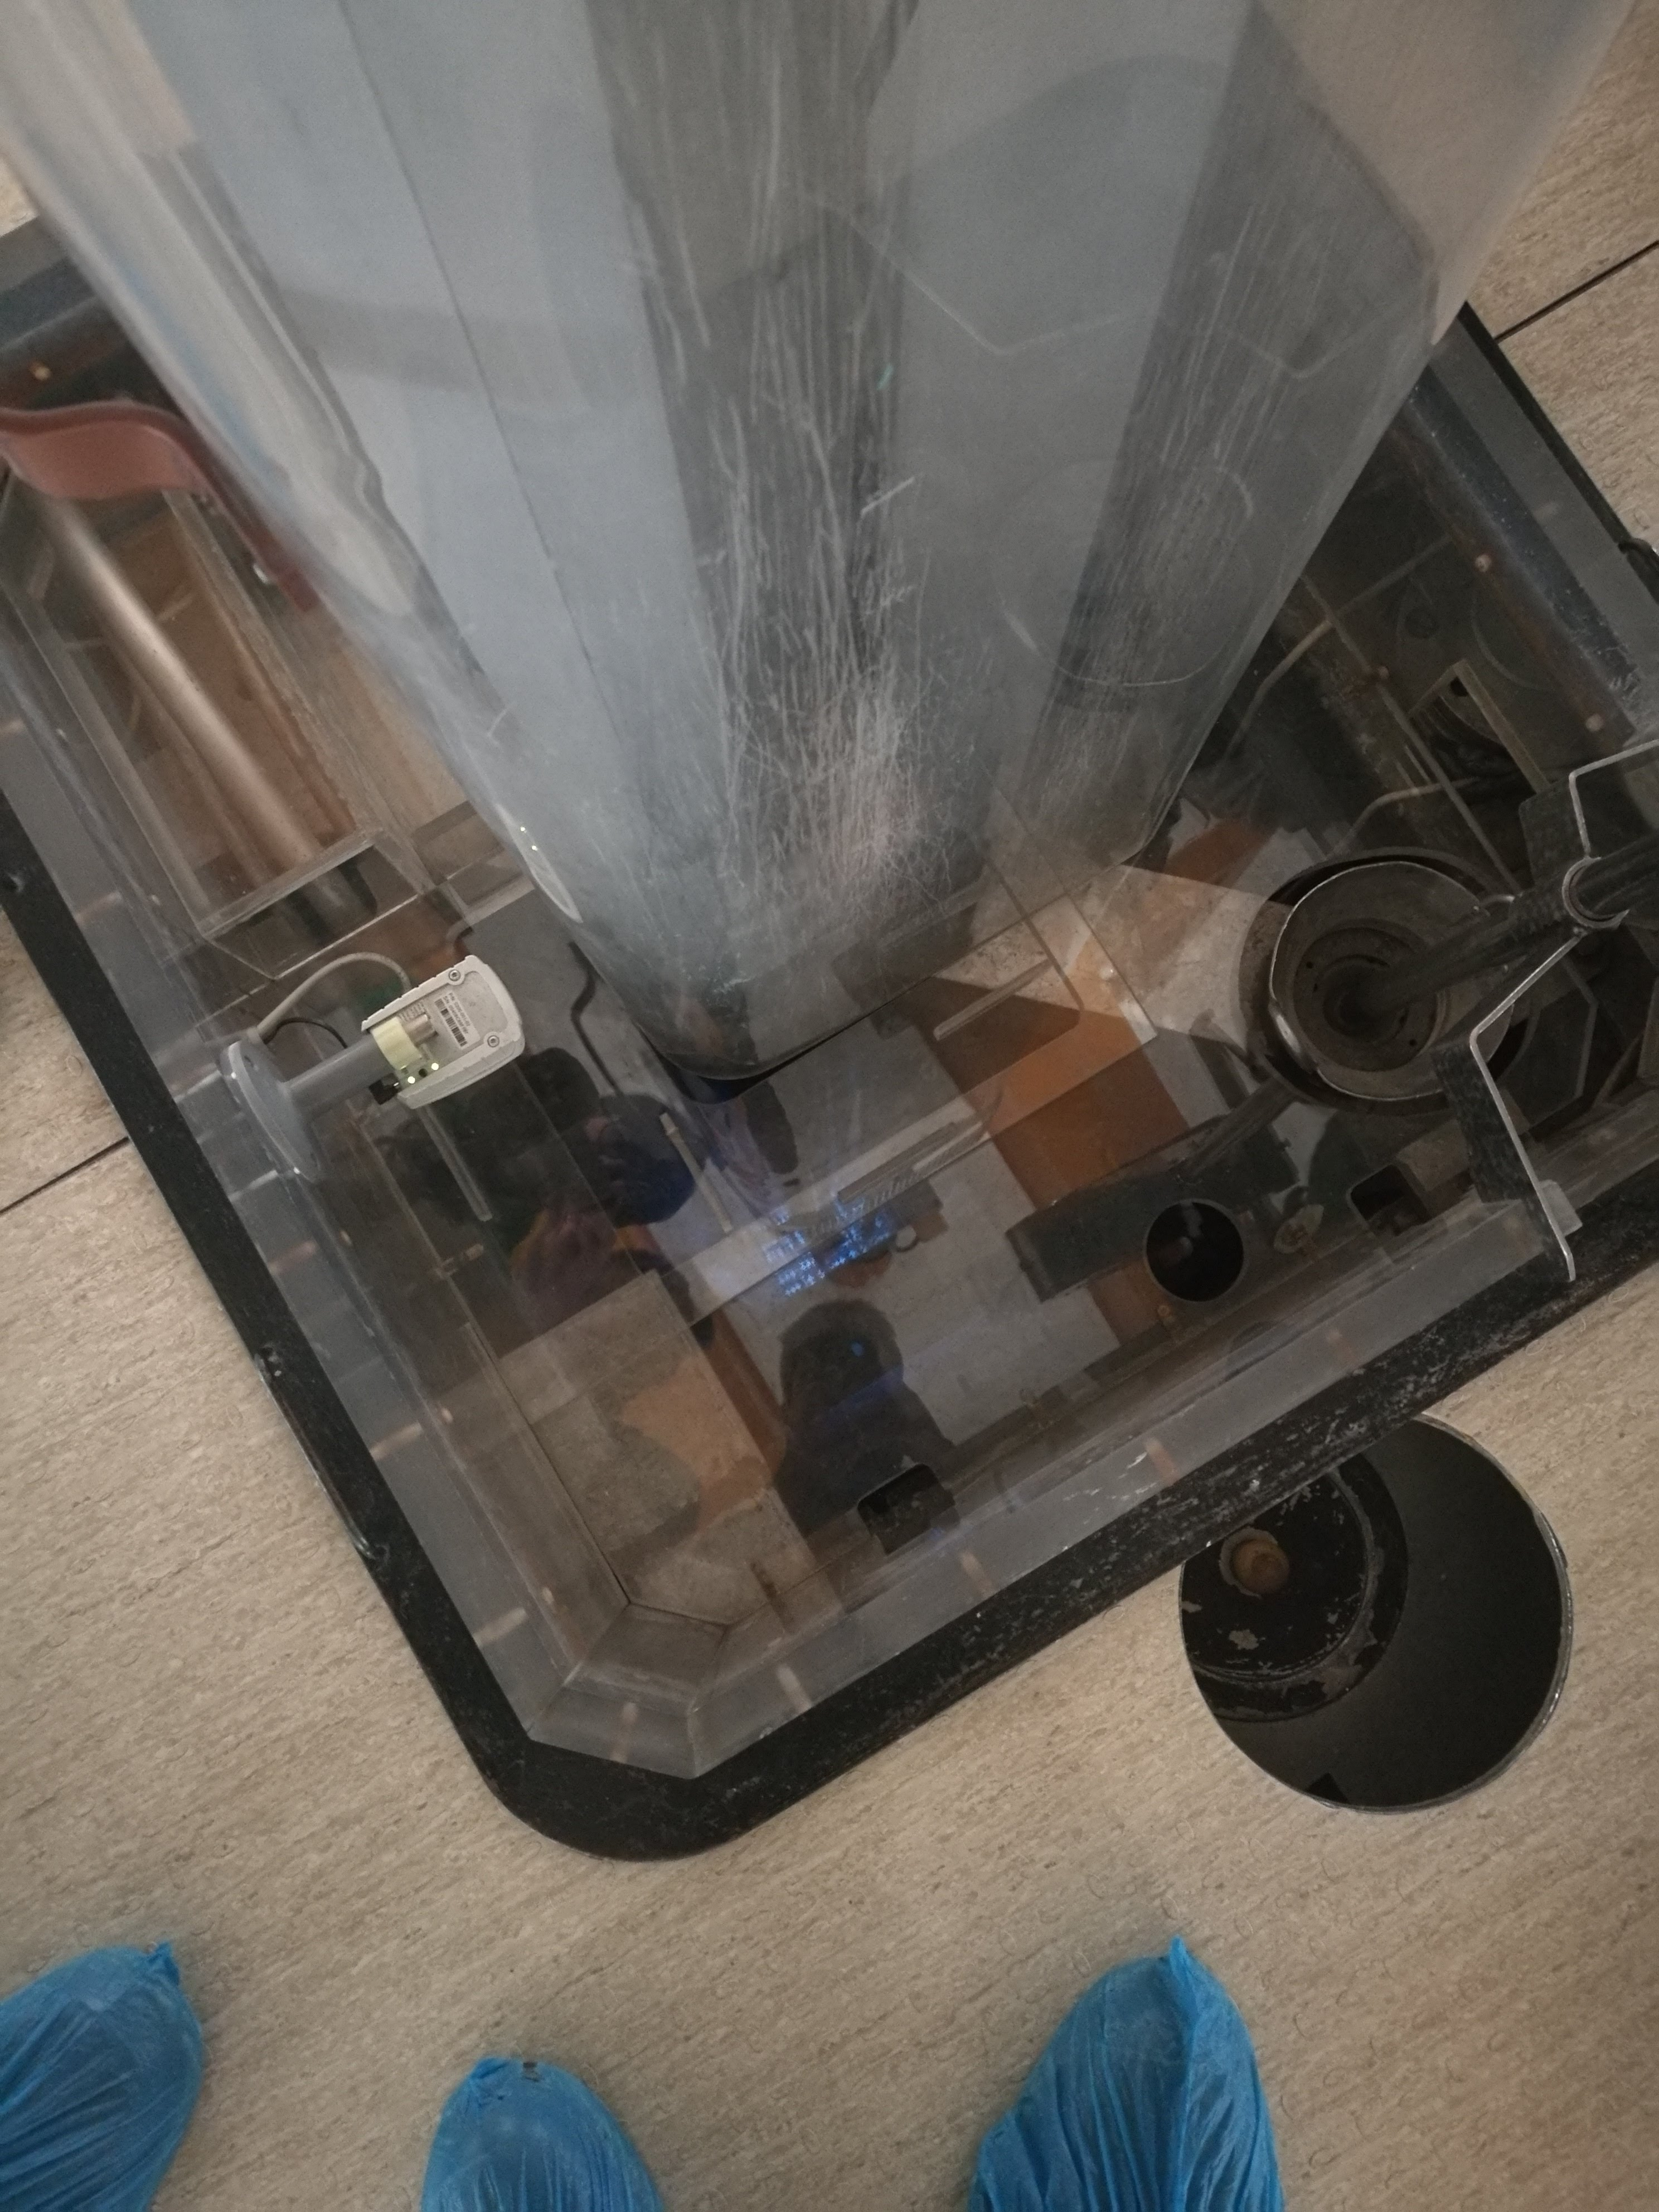
\includegraphics[width=0.48\textwidth]{../data/cherenkov.jpg}
\end{center}

\section{Összefoglalás}

\par Az idei laboratóriumi mérések mégha kifejezetten csak nehezítik is egy végzős hallgató mindennapjait, a mostani mérések kifejezetten értelmesek és hasznosak. Ezt a gyakorlatot egy élmény volt végigcsinálni. Maradandó emlék marad, amikor kamerával ténylegesen láttuk, hogy a reakció hirtelen leálltával megszűnik a Cserenkov-sugárzás.

\end{document}